\documentclass[a4paper,12pt]{article} % typ dokumentu i rozmiar czcionki

% Pakiety przydatne w fizyce
\usepackage[utf8]{inputenc}   % kodowanie pliku
\usepackage[T1]{fontenc}      % polskie znaki
\usepackage[polish]{babel}    % język dokumentu
\usepackage{amsmath, amssymb} % matematyka
\usepackage{graphicx}         % wstawianie obrazków
\usepackage{siunitx}          % poprawne jednostki
\usepackage{hyperref}         % linki w PDF
\usepackage{csvsimple}
\usepackage{booktabs}

\title{Linear Thermal Expansion Experiment} % tytuł raportu
\author{Roland Sobczak}
\date{\today} % data - automatycznie dzisiejsza

\begin{document}

\maketitle % generuje tytuł

\section{Introduction}

The aim of this experiment is to investigate the phenomenon of linear thermal expansion of solid materials and to determine the linear expansion coefficient of the tested material.

Thermal expansion is the change in the dimensions of a body due to a change in temperature. For small temperature changes, the length of a body changes proportionally to the temperature difference, according to the relation:
\begin{equation}
    \Delta L = \alpha \, L_0 \, \Delta T
\end{equation}
where:
\begin{itemize}
    \item $\Delta L$ – change in length,
    \item $L_0$ – initial length of the body,
    \item $\Delta T$ – temperature change,
    \item $\alpha$ – linear expansion coefficient.
\end{itemize}

This experiment allows us to verify this relationship and determine the value of $\alpha$ for a specific material, such as a metal, which is important when designing structures exposed to temperature variations.

\section{Experimental Procedure}

During the experiment, we measured the lengths of rods made from three different metals:
\begin{enumerate}
    \item Copper
    \item Brass
    \item Steel
\end{enumerate}

The procedure was as follows:

\begin{enumerate}
    \item First, we measured the initial absolute length of each rod. The measuring device had an accuracy of 0.05 mm. The initial temperature was 24.2°C.
    
    \item Next, we increased the temperature in steps of 5°C and measured the change in length relative to the initial length. For these measurements, the device had an accuracy of 0.01 mm. 
    
    \item For simplification, the measurements were performed at slightly different temperatures for each rod. Therefore, in the results section, the exact temperature for each measurement will be reported. The thermometer measured the temperature with an accuracy of 0.1°C.
\end{enumerate}

\section{Wyniki}

Tutaj przedstawiono wyniki pomiarów oraz wyliczone współczynniki rozszerzalności liniowej dla trzech metali.

\begin{figure}[h]
    \centering
    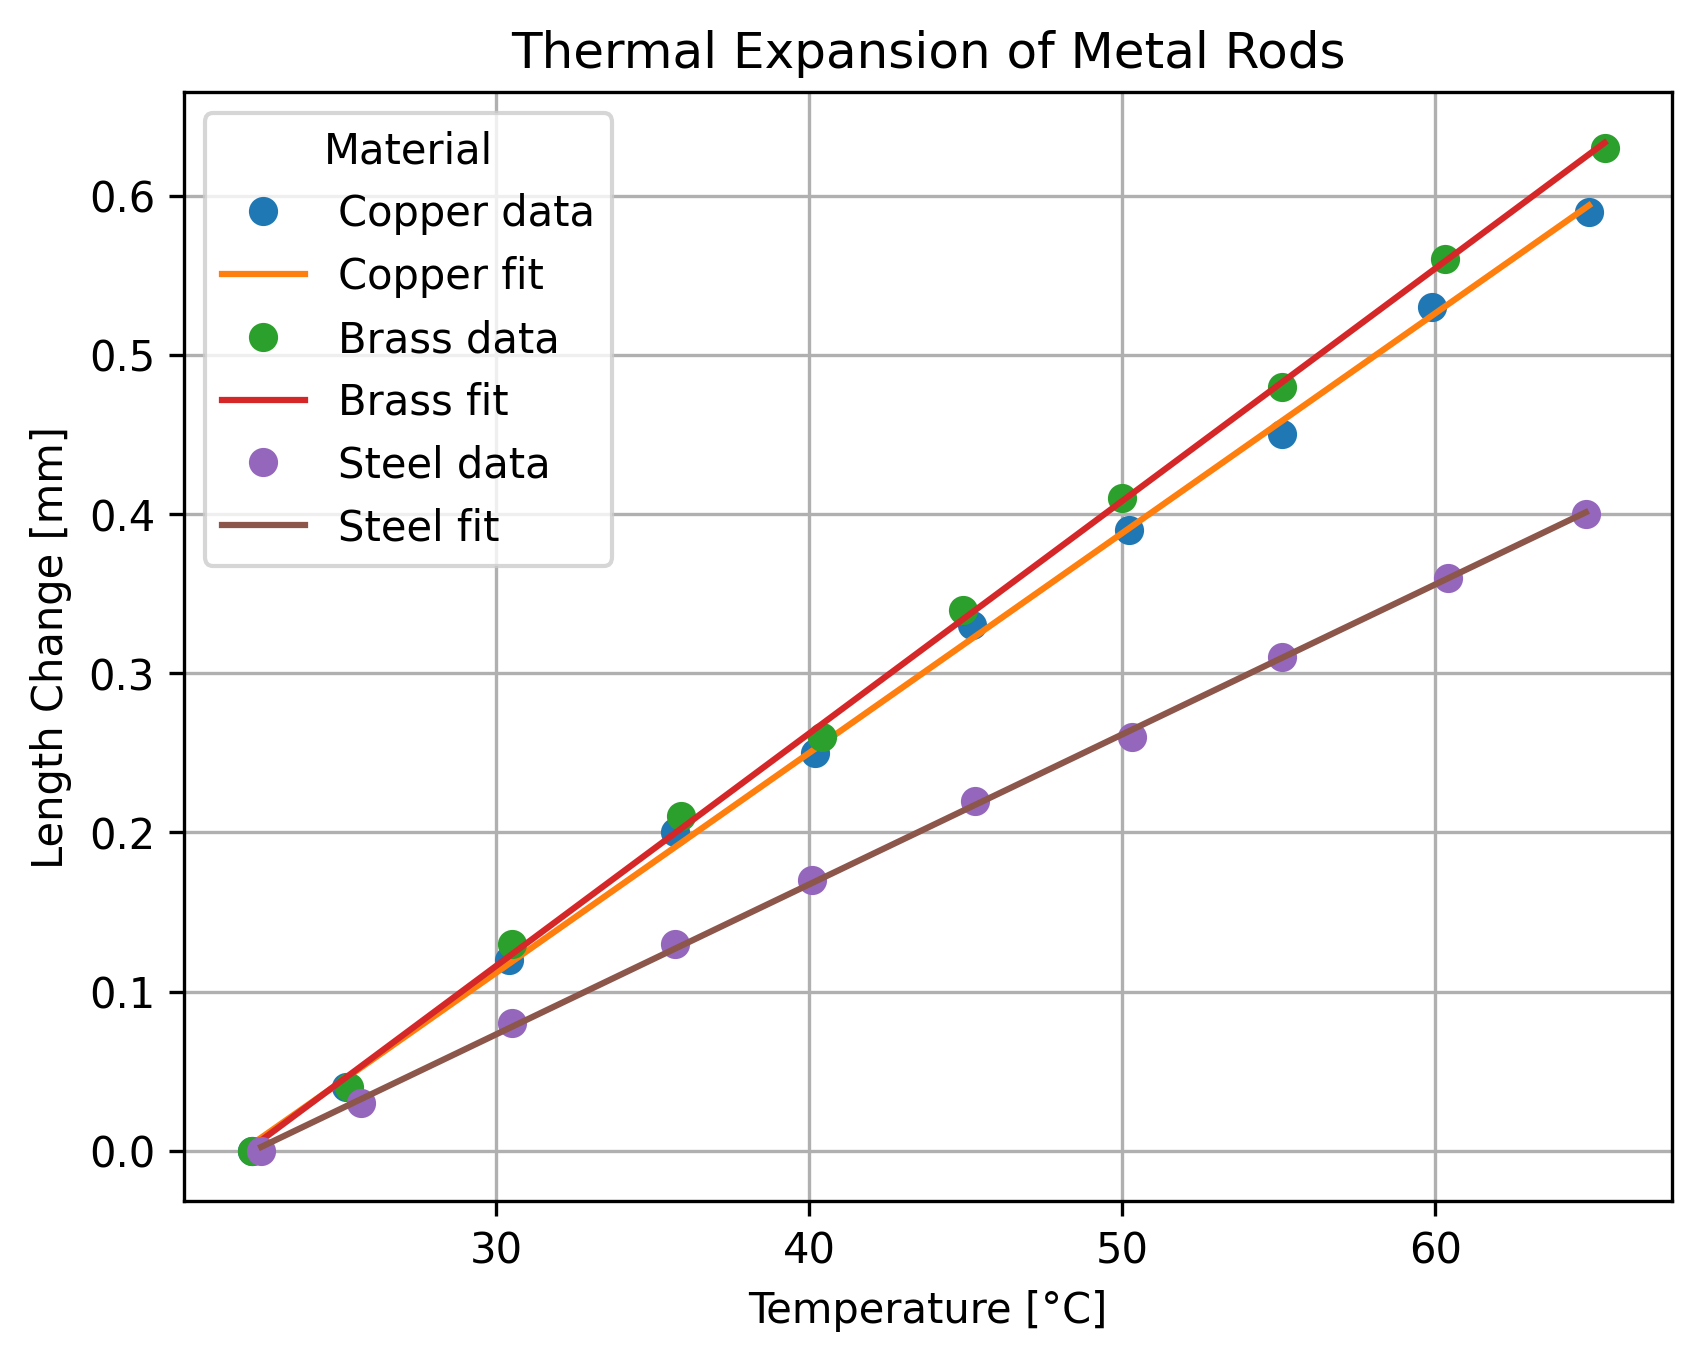
\includegraphics[width=1\textwidth]{expansion_plot.png}
    \caption{Thermal expansion of metal rods.}
    \label{fig:expansion_plot}
\end{figure}

\subsection*{Wyznaczone współczynniki}

\begin{tabular}{l c c}
\toprule
Metal & a [mm/°C] & $\alpha$ [1/°C] \\
\midrule
Copper & 0.013813 & $1.791 \cdot 10^{-5}$ \\
Brass  & 0.014608 & $1.894 \cdot 10^{-5}$ \\
Steel  & 0.009425 & $1.219 \cdot 10^{-5}$ \\
\bottomrule
\end{tabular}

\subsection*{Pełne dane pomiarowe}

\csvautotabular[respect all]{measurmentsout.csv}

\section{Wnioski}
Tutaj wpisujesz wnioski z doświadczenia.

\end{document}

